\documentclass{article}

% Language setting
% Replace `english' with e.g. `spanish' to change the document language
\usepackage[english]{babel}

% Set page size and margins
\usepackage[letterpaper,top=2cm,bottom=2cm,left=3cm,right=3cm,marginparwidth=1.75cm]{geometry}

% Useful packages
\usepackage{amsmath}
\usepackage[font=small,labelfont=bf]{caption}
\usepackage{graphicx}
\usepackage{microtype}
\usepackage[colorlinks=true, allcolors=blue]{hyperref}

\graphicspath{{figures/}}
\newcommand{\figref}[1]{Fig.~\ref{#1}}

\title{Reset as a Targeting Problem in Recurrent Spiking Networks}
\author{Jack Large, Jasper Mark}

\begin{document}
\maketitle

\begin{abstract}
Electrical stimulation can suppress the output of an adaptive neural network without erasing the synaptic changes that support learned behavior. We tested whether open-loop stimulation delivered through a simulated 64-channel multielectrode array could reset recurrent spiking networks trained on six families of electrode-association tasks. Reset was defined as a paired combination of behavioral forgetting, movement toward the pretraining synaptic state, loss of relearning savings, and preserved capacity to relearn. Across 50 network initializations per task and 60 stimulation protocols per task, no protocol satisfied reset as defined. The strongest chirp protocols produced the largest behavioral dents and moved weights by 2.2--5.1 times the learned trace norm, but their displacement was nearly orthogonal to the erasure direction: mean signed cosines were 0.002--0.030, corresponding to angles of 88.3--89.9 degrees. PCA/SVD of training-induced channel-pair weight changes showed a reproducible shared direction, with the first uncentered component explaining 77.7--86.8\% of variance, but residual structure was not one-dimensional: centered effective dimensionality was 11.0--24.8 and 10--21 principal components were required to explain 80\% of centered variance. Interpolation from trained toward naive weights crossed criterion only after reversing 81--94\% of the training-associated change, whereas matched random directions never crossed criterion. Ablations localized behavioral dependence to broader fan-out from input-electrode neurons and fan-in to target-electrode neurons rather than to bulk weight displacement or direct input-to-target edges alone. Thus, in this model and class of task, open-loop stimulation failed because it produced large weight motion in behaviorally insensitive directions. Reset is therefore a targeting problem.
\end{abstract}

\section{Introduction}

Dissociated neuronal cultures and engineered spiking networks are attractive experimental substrates because they combine recurrent dynamics, plasticity, and direct electrical access. Cultured networks can express stimulus-specific changes and pathway-dependent potentiation or depression under multielectrode-array (MEA) stimulation (CITATION NEEDED). At the same time, the literature shows that stimulation-induced plasticity can be difficult to establish with a behavioral readout that excludes drift and transient excitability changes (CITATION NEEDED). These difficulties become more apparent when the experimental objective is not learning but rather unlearning: returning an already trained adaptive substrate to a state that no longer expresses the learned mapping and can be trained again.

A drop in evoked output is not, alone, evidence of true unlearning (also referred to as a reset). Stimulation may transiently suppress spiking, alter membrane variables, or move many synaptic weights while leaving the task-supporting trace intact. Conversely, a network need not return to parity with its pretraining state to lose a memory; it could enter another task-neutral retrainable state. A defensible reset assay therefore needs several criteria in convergence. In the present study, behavioral forgetting is paired with a simulation-only measure of return toward the pretraining synaptic state and with a functional test based on relearning savings. The pretraining-weight overwrite is used as a positive control because it isolates the contribution of synaptic weights while preserving all other simulated state variables.

The central hypothesis of this study is rooted in the geometric nature of the network. In a high-dimensional recurrent network, large perturbations can be behaviorally weak when they point along insensitive directions. Related work in neural population dynamics and network control has shown that accessible directions can constrain learning and state transitions (Sadtler et al., 2014; Gu et al., 2015). Here, the same principle is tested in synaptic weight space under a deliberately asymmetric information constraint: the complete state is available for mechanistic analysis only, while stimulation and readout are restricted to the electrode interface, as they would be in a culture experiment.

We screened temporal, spatial, and spectral stimulation across six electrode-association task families. The screen produced sizable synaptic perturbations but no genuine reset. Three privileged analyses then separated magnitude, direction, and dimensionality. First, equal-norm movement toward the pretraining state and along random orthogonal directions produced sharply different behavioral outcomes. Second, PCA/SVD of training-induced channel-pair weight changes quantified the reproducibility and effective dimensionality of the learned weight changes across seeds. Third, targeted ablations showed that performance depended on input-electrode fan-out and target-electrode fan-in rather than on bulk weight magnitude or direct input-to-target edges alone. The resulting claim is that within the tested model, task family, and open-loop actuator space, reset is primarily a targeting problem.


\section{Methods}

\subsection*{Network model}

We simulated a dissociated cortical culture as a spatially embedded recurrent network of leaky integrate-and-fire neurons. Neurons were placed at random positions on a planar field and assigned excitatory or inhibitory identity with fixed probability. Connectivity was distance-biased: each neuron projected to a set of nearby targets drawn with probability decaying exponentially in inter-neuronal distance, supplemented by a sparse population of long-range recurrent connections. Excitatory synapses were plastic under a fixed-sign spike-timing-dependent plasticity rule with separate potentiation and depression time constants, and a slow homeostatic mechanism rescaled excitatory weights toward a target population firing rate. Synaptic signs were fixed at initialization and preserved under all subsequent manipulations, so that no analysis or perturbation could convert an excitatory synapse into an inhibitory one or vice versa. All reported experiments used networks of $10^4$ neurons. The full synaptic weight vector and all spike times were retained for analysis, but neither was accessible to the stimulation or readout pathway.

\subsection*{Electrode interface and behavioral task}

The network was actuated and observed only through a simulated 64-channel multielectrode array, mirroring the constraints of a wetware culture. Stimulation entered the network as charge-balanced pulse events delivered to electrode channels, each event driving the subset of neurons nearest that channel. Observation was limited to channel-level multi-unit activity: per-channel spike counts and times pooled over the neurons assigned to each electrode. The learned task was an electrode-to-electrode conditioned association. During training, input-electrode pulses were paired with target-electrode pulses at fixed delays, and native plasticity strengthened pathways that made target responses follow the relevant inputs. We studied six electrode-association task families: single conditioned association, two-pattern discrimination, overlapping shared-target mappings, overlapping shared-input mappings, multi-association mappings, and XOR-like electrode classification. Networks were trained to a behavioral criterion or for a fixed maximum number of repetitions, whichever came first.

\subsection*{Behavioral readout and its controls}

The behavioral score was defined as the difference between the response probability on positive (trained) probes and the response probability on negative or cross probes, evaluated with plasticity disabled and averaged over repeated probe presentations from identical cloned states. Before using this score to evaluate reset, we required it to pass two controls. First, the score had to be input-specific: a trained network must respond to the genuine input pulse but not to a matched sham probe. Second, and most stringently, the score had to be weight-dependent: overwriting the trained synaptic weights with the pre-training (naive) weights, while leaving every other state variable intact, had to return the score to chance. This naive-weight overwrite served throughout as the privileged positive control --- the one manipulation guaranteed to remove the learned synaptic trace, and the ceiling against which stimulation was compared.

\subsection*{Paired-clone reset assay}

Reset was evaluated by a within-state paired comparison. For each network seed and task, we trained once to criterion and then cloned the entire trained state, including synaptic weights, membrane variables, plasticity traces, and homeostatic variables. From this clone we ran two matched branches: a reset branch, which received a candidate stimulation protocol, and a no-reset branch, which received an equal duration of plasticity-on rest. Behavioral score, synaptic state, channel activity, and subsequent relearning were measured on both branches, so that every reported effect of stimulation is a difference between two branches descended from the same trained state.

\subsection*{Stimulation protocol space}

Candidate reset protocols were drawn from a coarse grid spanning three actuator axes expressible through the electrode interface: the temporal color of the stimulation (spectral slope of event timing, from blue through white to red/brown), the schedule (static, alternating-color, epoch--pause, chirp, and gated-burst structures), and the spatial pattern across channels (shared, independent, correlated, or phase-shifted). Stimulation current, pulse width, duration, and pulse count were tracked as cost variables. The grid was a screen of the reachable actuator space rather than an optimization, and protocols were expressed as electrode pulse trains rather than as direct current injection into individual neurons.

\subsection*{Outcome measures: apparent, mechanistic, and functional reset}

We distinguished three operationally separate senses of reset. Apparent reset was a reduction of the post-stimulation behavioral score relative to the matched no-reset branch. Mechanistic reset was movement of the synaptic weight vector back toward the naive state; we quantified both the displacement magnitude relative to the no-reset branch and the signed projection of that displacement onto the training-defined synaptic axis, defined as the difference between the trained and naive weight vectors. We also converted this projection into a signed cosine with the erasure direction, $\cos\theta = \langle W_{\mathrm{reset}} - W_{\mathrm{rest}}, W_{\mathrm{naive}} - W_{\mathrm{trained}}\rangle / (\|W_{\mathrm{reset}} - W_{\mathrm{rest}}\|\,\|W_{\mathrm{trained}} - W_{\mathrm{naive}}\|)$. This axis is available only in simulation, where the full weight state and the pre-training state are known, and was used for mechanistic interpretation rather than as a biologically observable control signal. Functional reset was a reduction in relearning savings, defined as one minus the ratio of relearning repetitions to initial-learning repetitions, so that a protocol that left no savings would require as many repetitions to retrain as to train initially. A protocol counted as a genuine reset only if it improved all three measures while leaving the network able to relearn.

\subsection*{Memory-geometry analyses}

To localize the learned trace in weight space, we performed three analyses on trained networks, exploiting the fact that the synaptic state is observable in the model even though it is hidden from the actuator. First, we measured the breaking point along the training-defined memory axis by interpolating the weight vector between the trained and naive states, $W(\alpha) = (1 - \alpha)\,W_{\mathrm{trained}} + \alpha\,W_{\mathrm{naive}}$, and reading the behavioral score as a function of $\alpha$; the breaking point $\alpha^{*}$ was the smallest fraction of the way to naive at which the score fell below criterion. As a control we displaced the weights by the same magnitude along a random direction orthogonal to the training-defined axis. Second, we aggregated each seed's training-induced weight change, $W_{\mathrm{trained}} - W_{\mathrm{naive}}$, into a fixed 64-by-64 channel-pair representation and ran PCA/SVD across seeds within each task. We report variance explained, participation-ratio effective dimensionality, pairwise seed angles, and the number of principal components required to explain 80\% and 90\% of centered variance. Third, we performed surgical ablations against the validated readout, zeroing or scrambling defined synapse sets --- the input-to-target pathway, all edges incoming to target-electrode neurons, all edges outgoing from input-electrode neurons, a magnitude-preserving shuffle, and a magnitude-matched random displacement --- to test whether these electrode-association tasks are stored in a localized set of electrode-defined connections or distributed across the network.

\subsection*{Statistics and reproducibility}

The independent experiment was the network seed within task. The reset screen was replicated across 50 network seeds per task and 60 protocols per task; reported screen summaries use mean, standard deviation, and 95\% confidence intervals across protocol--seed trials or across seeds where stated. Memory-geometry interpolation, surgical ablation, and PCA/SVD analyses were run across 50 seeds per task. PCA uncertainty was estimated by bootstrap resampling seeds 1,000 times. Reset effects were evaluated as paired differences between the reset and no-reset branches of a common clone, and these paired score differences are the behavioral effect sizes used throughout. Behavioral scores were averaged over repeated plasticity-off probe presentations. All networks, protocols, and analyses were generated from fixed random seeds and are fully reproducible from the recorded run configuration.

\section{Results}

\subsection*{Validation of the behavioral readout}

Networks of $10^{4}$ neurons learned electrode-to-electrode associations to criterion within tens of training repetitions. Before using behavior to evaluate reset, we required the readout to pass two controls. The score was input-specific, distinguishing genuine input pulses from matched shams only after training, and it was weight-dependent: overwriting the trained weights with the pre-training weights while leaving all other state intact returned the score to chance (\figref{fig:task-assay}). This naive-weight overwrite --- the one manipulation guaranteed to remove the synaptic trace --- served throughout as the privileged positive control and the ceiling against which stimulation was compared.

\begin{figure}[t]
  \centering
  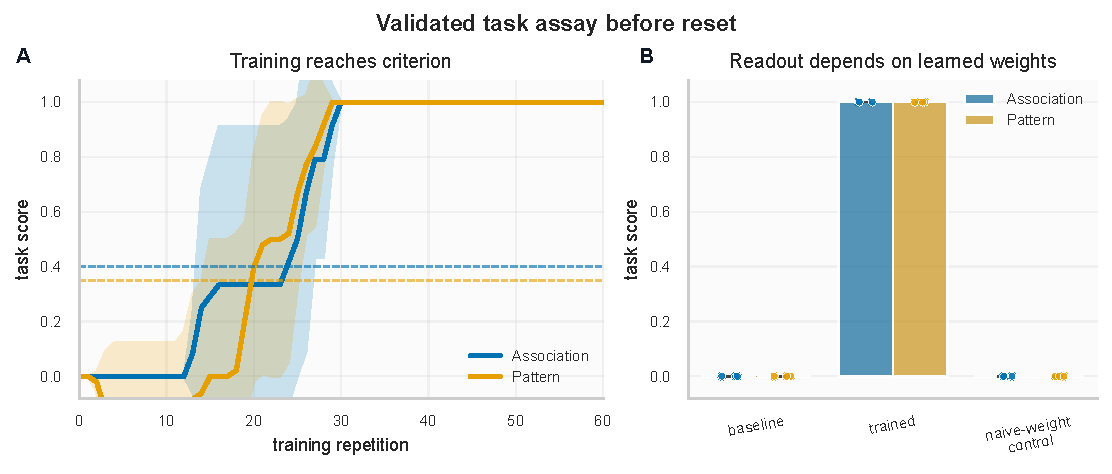
\includegraphics[width=\linewidth]{fig1_design.pdf}
  \caption{\textbf{Validated task assay before reset.}
  \textbf{A,} Training histories for the association and pattern-discrimination tasks, with dashed lines marking the task-specific criterion.
  \textbf{B,} The behavioral readout separates trained networks from baseline and from the naive-weight control, showing that the measured task score depends on the learned synaptic weights.
  Points denote network seeds and bars show the mean with seed-wise spread.}
  \label{fig:task-assay}
\end{figure}

\subsection*{Perturbation without reset}

Across the 50-seed coarse protocol grid, no stimulation branch met the forgetting criterion in any task. The strongest protocol in each task was a high-amplitude chirp and produced only partial apparent forgetting: mean forgetting scores were 0.125 for association, 0.528 for pattern discrimination, 0.372 for shared-target mappings, 0.094 for shared-input mappings, 0.245 for multi-association mappings, and 0.075 for XOR. These protocols moved the reset branch by 2.2--5.1 memory-trace norms, but the displacement was almost perpendicular to the erasure direction: mean absolute cosines were 0.004--0.030, mean signed angles were 88.3--89.9 degrees, and the orthogonal fraction of displacement was 0.9995--1.000. Across all protocol--seed trials with nonzero weight movement, the median absolute cosine was only 0.006--0.016 depending on task. Relearning savings persisted after stimulation, indicating preserved functional memory rather than genuine reset (\figref{fig:functional-dissociation}; \figref{fig:weight-geometry}).

\begin{figure}[t]
  \centering
  
\includegraphics[width=\linewidth]{fig2_readout.pdf}
  \caption{\textbf{Protocol screen: stimulation burden is not reset.}
  \textbf{A,B,} Mean immediate forgetting across schedule and temporal-color settings for the association and pattern-discrimination tasks.
  \textbf{C,} Extra reset-window spiking and delivered charge increase stimulation burden but do not produce a reliable return to chance behavior.
  The screen spans protocols reachable through the 64-channel electrode interface.}
  \label{fig:protocol-screen}
\end{figure}

\begin{figure}[t]
  \centering
  
\includegraphics[width=\linewidth]{fig3_dissociation.pdf}
  \caption{\textbf{Functional memory survives the reset sweep.}
  \textbf{A,} Reset-induced weight motion has near-zero signed cosine with the erasure direction, indicating almost entirely off-axis displacement.
  \textbf{B,} Large total synaptic displacements leave post-reset task scores above criterion.
  \textbf{C,} Relearning remains faster than initial learning after stimulation, indicating preserved functional memory rather than genuine reset.}
  \label{fig:functional-dissociation}
\end{figure}

\begin{figure}[t]
  \centering
  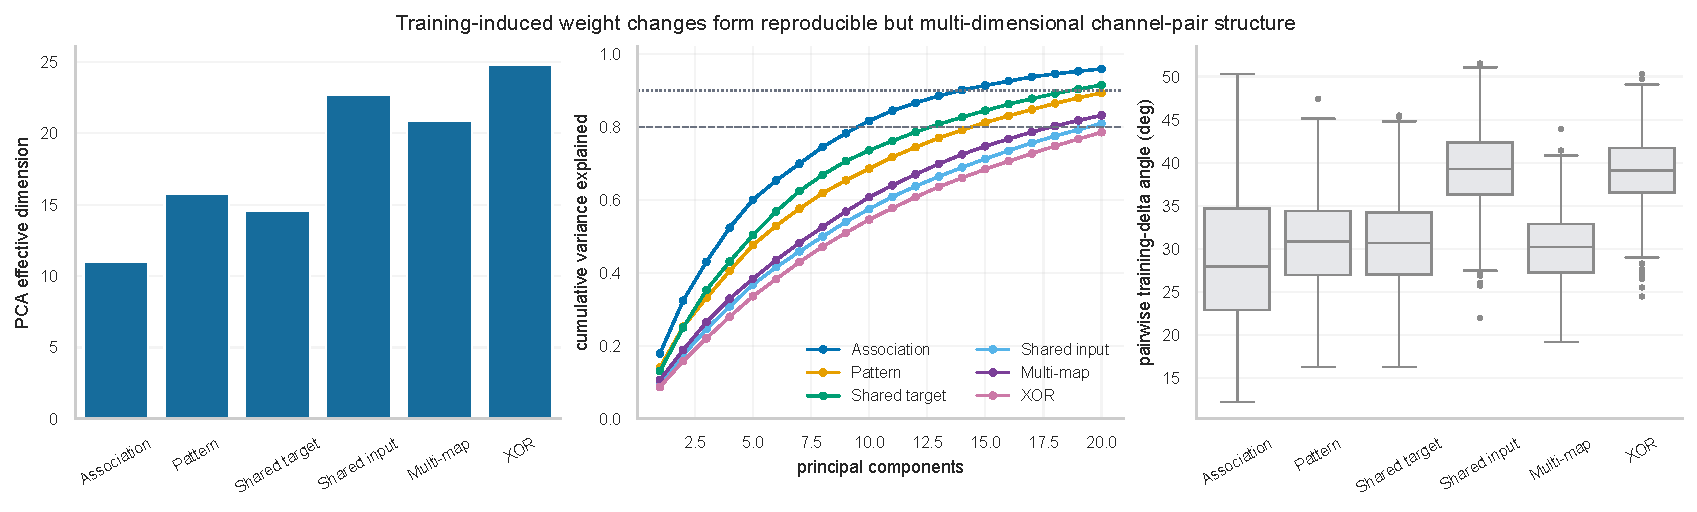
\includegraphics[width=\linewidth]{fig6_weight_pca_dimensionality.pdf}
  \vspace{0.6em}
  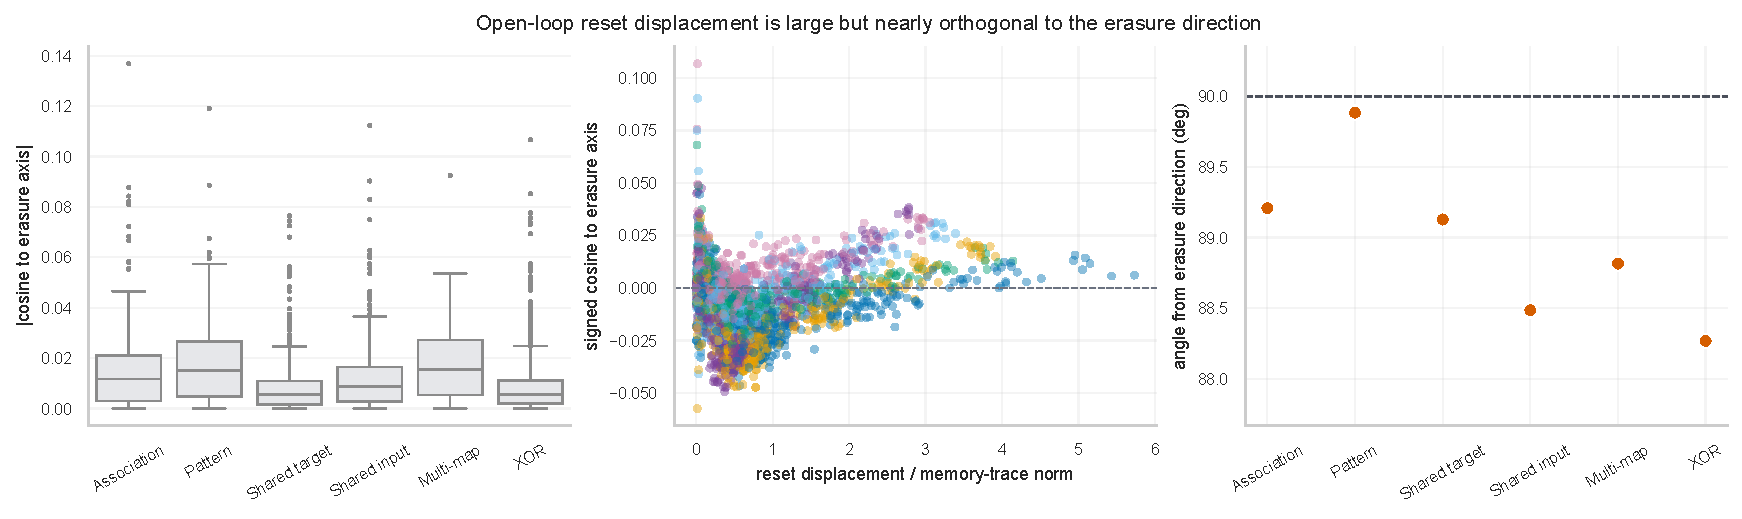
\includegraphics[width=\linewidth]{fig6_reset_axis_orthogonality.pdf}
  \caption{\textbf{Quantitative weight-space geometry of learning and reset.}
  Top, PCA/SVD of seed-wise training-induced channel-pair weight changes shows a strong shared direction but residual multi-dimensional structure.
  Bottom, reset displacements have small absolute cosine with the erasure direction; the strongest protocol in each task remains near 90 degrees from that direction.}
  \label{fig:weight-geometry}
\end{figure}

\subsection*{Direction versus magnitude of weight change}

Across 50 seeds per task, interpolation toward the naive state crossed criterion only after reversing most of the training-associated change: mean $\alpha^{*}$ was 0.81 for association, 0.83 for pattern discrimination, 0.82 for shared-target mappings, 0.94 for shared-input mappings, 0.83 for multi-association mappings, and 0.85 for XOR classification (\figref{fig:breaking-point}). Matched random directions never crossed criterion in any seed or task. Sensitivity to weight movement therefore depended strongly on direction: the network tolerated large untargeted displacement while requiring targeted reversal along the training-defined axis to collapse behavior.

PCA/SVD showed that training-induced weight changes were reproducible but not one-dimensional. The first uncentered component explained 77.7--86.8\% of variance, reflecting a strong shared task-aligned direction across seeds. After centering, however, PC1 explained only 8.7--17.9\%, the top five PCs explained 33.6--60.0\%, and participation-ratio effective dimensionality ranged from 11.0 to 24.8. Depending on task, 10--21 PCs were needed to explain 80\% of centered variance and 14--29 PCs were needed to explain 90\% (\figref{fig:weight-geometry}).

\begin{figure}[h]
  \centering
  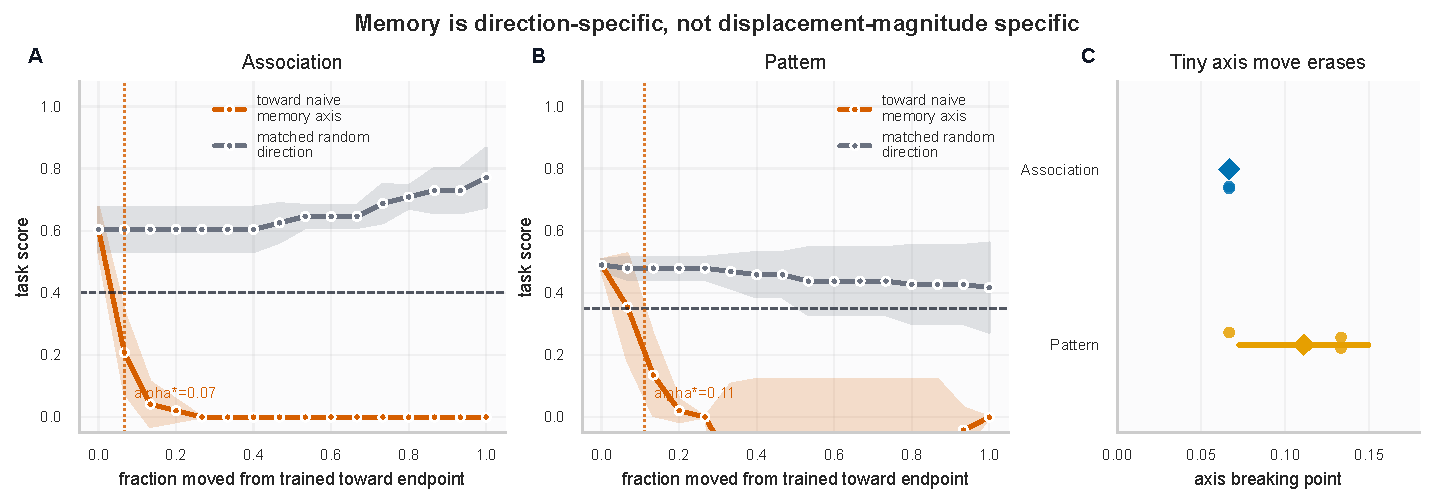
\includegraphics[width=\linewidth]{fig4_breaking_point.pdf}
  \caption{\textbf{Task performance is direction-specific rather than displacement-magnitude specific.}
  \textbf{A,B,} Moving weights toward the naive state along the training-defined memory axis rapidly collapses performance, whereas matched random orthogonal displacement preserves the task score.
  Dashed horizontal lines mark criterion and dotted vertical lines mark the axis breaking point.
  \textbf{C,} Seed-wise breaking points show that erasure requires directed movement along the training-defined axis, while matched random displacements do not cross criterion.}
  \label{fig:breaking-point}
\end{figure}

\subsection*{Localization of the memory trace}

Surgical ablations against the validated readout localized task dependence to broader electrode-defined pathways rather than to bulk recurrent magnitude or direct input-to-target edges alone (\figref{fig:ablations}). Removing all outgoing edges from task input channels or all incoming edges to task target channels reduced performance to near chance across tasks, while direct task-path removal alone was comparatively weak and matched random displacements preserved performance. For these electrode-association tasks, the learned representation is therefore concentrated in input- and target-associated pathway structure, not in bulk synaptic strength or a single direct edge set.

\begin{figure}[!h]
  \centering
  
\includegraphics[width=\linewidth]{fig5_ablations.pdf}
  \caption{\textbf{The learned association is pathway-specific.}
  \textbf{A,} Targeted pathway perturbations abolish task performance, while magnitude-preserving shuffles and magnitude-matched random displacements do not.
  Dashed lines mark task criteria.
  \textbf{B,} The effective pathway perturbations alter only a small fraction of synapses, showing that memory is concentrated in input- and target-associated pathway structure rather than bulk recurrent weight magnitude.}
  \label{fig:ablations}
\end{figure}

\subsection*{A geometric account of reset failure}

Together these results explain why open-loop stimulation suppresses behavior without erasing memory. Training creates a reproducible shared direction in channel-pair weight space, but behavior is sensitive to movement along a specific erasure direction that open-loop stimulation largely misses. Large reset displacements remain almost perpendicular to that direction, explaining why stimulation can perturb activity and weights without erasing the learned mapping. Reset is therefore not only a question of stimulation strength but also of targeting, suggesting that successful reset may require closed-loop control capable of selectively perturbing task-relevant synaptic subspaces.

\subsection*{Limitations and biological scope}

The present work should be interpreted as a mechanistic study in a simplified recurrent spiking model rather than a direct model of cultured cortical networks. The model uses leaky integrate-and-fire neurons, pair-based spike-timing-dependent plasticity, and homeostatic scaling; it does not include conductance-based cellular dynamics, heterogeneous cell classes beyond excitatory/inhibitory identity, experimentally measured connectivity distributions, or the full biophysics of dissociated cultures. Accordingly, the biological claim is limited: the simulations show that an electrode-constrained recurrent SNN can preserve a learned association under large open-loop perturbations when those perturbations miss the task-relevant synaptic direction. Whether the same geometry appears in CL1 cultures must be tested with closed-loop wetware experiments and richer model variants.

Two additional limitations follow from the task and analysis design. First, the primary tasks are electrode associations, so pathway-specific storage may partly reflect the input-to-target structure of the task. We therefore frame the localization result as evidence for pathway-specific representations in these electrode-association tasks, not as a general claim that all recurrent SNN memories share this geometry. Second, the memory axis is a privileged simulation-only quantity, $W_{\mathrm{trained}} - W_{\mathrm{naive}}$, available because the model exposes the full trained and naive weight states. Likewise, the PCA/SVD analysis uses a simulation-derived channel-pair representation that is comparable across random network seeds; it is mechanistic rather than directly observable in wetware. A biological reset controller would still need to estimate analogous task-relevant directions from electrode-level responses rather than from privileged access to synaptic weights.

\end{document}
